\section{Data}
\label{sec:data}

\subsection{Choosing the objects}
\label{sec:cohort}

The main sample is 250 passive objects between 400 and 800~km. We kept objects that appear on at
least eight of nine Space-Track snapshot dates and spread the sample across 100-km altitude bands
instead of picking by NORAD number, which gives 39, 63, 82 and 66 objects in the four bands. We
use debris and rocket bodies because they cannot correct their orbits. We also kept 15 objects
between 1,040 and 1,211~km as a high-altitude control group, since storms should barely touch
them. The first full download gave 205,145 deduplicated TLE states and 199,580 intervals between
neighbouring states: 188,560 in the main sample and 11,020 in the control group.

For the operator question we built a separate active cohort of 25 Starlink satellites and 25
other payloads, chosen with the same coverage rule. Their pipeline keeps station-keeping
intervals and does not remove climbs. The joined object catalogue has 291 objects.

\subsection{Cleaning the TLEs}
\label{sec:cleaning}

We parse each TLE with SGP4~\cite{vallado2006sgp4} and convert its (Kozai) mean motion to a mean
semi-major axis using the WGS-72 constants. Using SGP4's recovered (Brouwer) mean motion instead
shifts the semi-major axis by a nearly constant amount of up to about 3~km and changes decay
rates by 0.03\% over the cohort (at most 0.2\% for any object), so nothing depends on this choice. When the same epoch was published
more than once we keep only the latest record, so that re-issues do not create fake intervals of
zero or near-zero length.

One point needs care, and a reviewer of our project proposal raised it directly. TLEs are mean
elements fitted to a day or more of tracking. They are not measured positions, so when we say
``altitude'' we mean the mean semi-major axis minus Earth's equatorial radius, not a true
geometric height. SGP4 fitting artifacts and changes in eccentricity can both create altitude
drops that never happened, and a storm study is exactly where such fake drops would do the most
harm. We defend against them in three ways. First, we track the mean semi-major axis rather than
perigee height, which swings with eccentricity, and we keep only near-circular orbits
(eccentricity below 0.01). Second, we reject states outside the altitude bounds, cross-tag
jumps, pairs that fail the TLE consistency checks at either end, and isolated jumps caught by a
Hampel filter. Third, for the largest storms we also compare calm-to-calm totals
(Section~\ref{sec:extreme}), which do not depend on how a fit spreads a loss across days.

Neighbouring clean states form an interval. We drop intervals that straddle a storm onset,
because they cannot be called either before or after the storm; 5,300 were dropped this way.
Four intervals were longer than five days (the longest 7.1 days), and we kept and reported them
rather than quietly removing them. The cross-tag and rolling-median checks flagged no objects.

TLE noise can make an object appear to climb a little. We estimate each object's noise level
from local median absolute deviations and flag such climbs, but keep them in the table, because
deleting only the upward steps would bias decay downwards. Dropping them anyway moves the
short-run storm effect only from $-14.1$ to $-14.6$~m/day. The outlier step is a Hampel filter
on the NRLMSIS~2.1 residual, with a five-day window and $k = 3.5$. It flags 11,005 passive
intervals in all (5.5\%), and these are left out of every analysis. In the main sample, 178,107
of the 188,560 intervals pass and form the analysis sample. Table~\ref{tab:cleaning} lists the steps.

\begin{table}[t]
\caption{TLE cleaning steps (passive cohort, first download)}
\label{tab:cleaning}
\centering
\small
\begin{tabular}{@{}p{2.55cm}p{2.45cm}p{2.5cm}@{}}
\toprule
Step & Affected & Treatment \\
\midrule
Deduplication & 205,145 states kept & Keep latest re-issue \\
Storm-onset bridge & 5,300 intervals & Dropped \\
Gap $>$5 days & 4 (max 7.1 d) & Reported, kept \\
Cross-tag check & 0 objects & None removed \\
Rolling median & 0 objects & None removed \\
Climb diagnostic & 4,705 intervals & Kept, flagged \\
Hampel filter & 11,005 (5.5\%) & Excluded \\
\bottomrule
\end{tabular}
\end{table}

The outcome for each interval is the change in semi-major axis divided by the elapsed time, in
metres per day, so a negative number means the object is coming down. Each row also carries the
storm it belongs to, its day relative to that storm's onset, its cleaning flags, altitude band
and object role, so every analysis applies the same exclusions without going back to the raw
TLEs.

\subsection{Do TLEs see storm decay?}
\label{sec:precise}

Before trusting TLEs, we compared them with precise orbits from GRACE-FO-1~\cite{landerer2020gracefo}
and Swarm-A~\cite{friis2006swarm}. These products give position and velocity directly. We turn
them into an osculating semi-major axis with the vis-viva equation, average over whole orbits and
then compute daily decay rates. For Swarm-A we measure the orbital period from successive radius
minima (93.83~min) instead of assuming it, and we remove duplicate timestamps at file boundaries.

The October 2024 GRACE-FO comparison is the clearest test. The TLE and precise decay rates peak
on the same day, correlate at about 0.70 with no lag, and have a similar storm-day size (about
$-0.10$ against $-0.12$~km/day). So TLEs catch the timing and most of the size of storm decay,
while slightly underestimating the peak. Over 19 days in May 2024, the semi-major-axis levels
agree with a centred correlation of 0.907, a centred RMSE of 0.097~km and a slope difference of
0.0025~km/day once the mean-versus-osculating offset is removed. Swarm-A gives a weaker
zero-lag correlation of 0.457. Its product and sampling are different, so we treat it as a
supporting check rather than pooling it with GRACE-FO. Together they show the cleaned TLE intervals are good enough for a cohort
study.

\subsection{Space weather and the storm list}
\label{sec:sw}

Space-weather data come from NASA OMNIWeb: the planetary index ap (3-hourly and linear in
disturbance, so it can be averaged), the Dst index, Kp, and the daily F10.7 flux with its 81-day
centred mean. We measure storm strength with ap or Dst and never average Kp, which is
quasi-logarithmic.

We call any period with Dst below $-50$~nT a storm and merge dips less than three days apart.
For each storm we record the main-phase onset (the hour of highest Dst in the 24~h before the
minimum), the minimum Dst, and the recovery end (the first hour after the last sub-$-50$~nT hour
at which Dst climbs back above $-30$~nT). By minimum Dst, storms are moderate ($-50$ to
$-100$~nT), strong ($-100$ to $-200$), severe ($-200$ to $-350$) or extreme (below $-350$). Our
window has 20 storms: 11 moderate, 6 strong, 2 severe (October 2024 and 31 December 2024) and 1
extreme (May 2024, Dst $-406$~nT). Day~0 is always the main-phase onset, and the event window
runs from day $-10$ to day $+20$.

Fig.~\ref{fig:may} shows the raw signal: around the May 2024 storm, the median
decay rate of the 250 passive objects goes from $-18$~m/day three days before onset to
$-60$~m/day on the first day after it.

\begin{figure}[t]
\centering
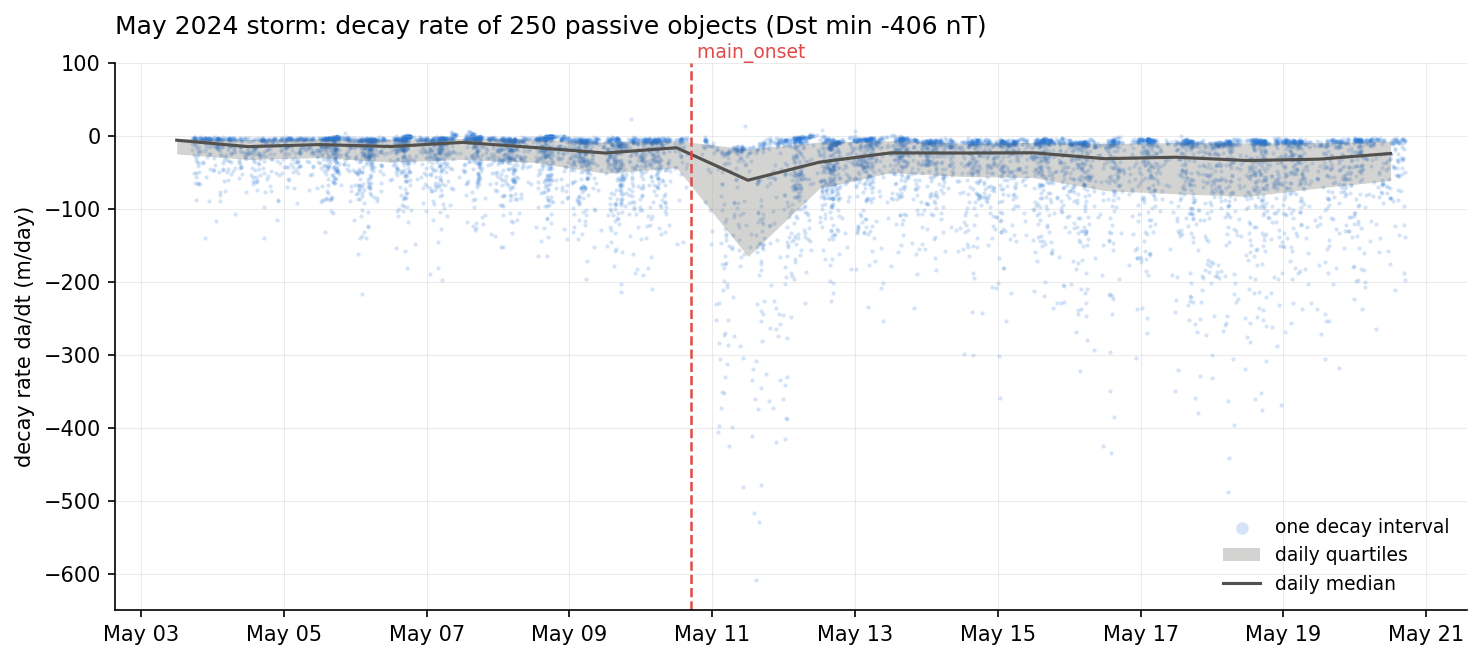
\includegraphics[width=\columnwidth]{fig1_may2024_cohort.png}
\caption{Median decay rate of the 250 passive objects around the May 2024 storm. Decay
increases about 3.4-fold on the first day after main-phase onset.}
\label{fig:may}
\end{figure}
